%!TEX root = main.tex

\newpage
\section*{About This Project}
\vspace{10mm}
\centerline{\textbf{Abstract}}

The field of cryptocurrency has enjoyed exponential growth in popularity in recent years. Almost ten years ago, the release of Bitcoin marked the beginning of a new era of innovation in the financial sector. In this dissertation we outline what exactly defines a cryptocurrency, describing fundamental concepts, underlying technologies such as the blockchain, and subsequently the viability of this new digital financial asset. Building on this knowledge, we examine the infamous volatility of cryptocurrency prices, analysing pricing data and the likelihood of these currencies, specifically Bitcoin, being in the midst a financial bubble. We examine the prediction of prices, or rather inability to do so, before introducing the Currency Analyser web application developed as part of this project. Containing up to date prices, this web application is hosted on Heroku for public access and predicts prices of Bitcoin using machine learning. The research, planning methodologies, technologies, and design and evaluation of this application are described in detail in the penultimate chapter of this dissertation, followed by a concluding word on the process as a whole.
\vspace{10mm}

\centerline{\textbf{Authors}}
\noindent This project was developed as a 15 credit project by Tara O'Kelly and Rebecca Kane, final year students of Software Development at Galway Mayo Institute of Technology. 
\begin{figure}[b]
\centering
\begin{minipage}{.5\textwidth}
  \centering
  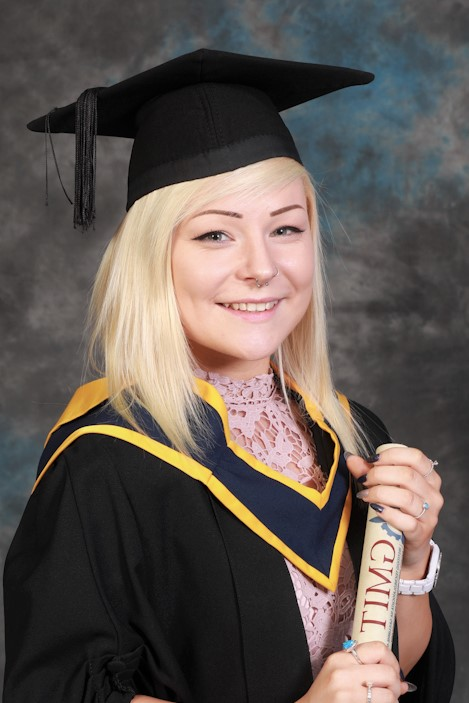
\includegraphics[width=.47\linewidth]{img/rebecca.jpg}
  \captionsetup{labelformat=empty}
  \caption{\textit{Rebecca Kane}}
\end{minipage}%
\begin{minipage}{.5\textwidth}
  \centering
  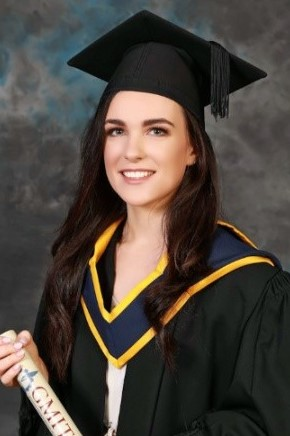
\includegraphics[width=.47\linewidth]{img/tara.jpg}
  \captionsetup{labelformat=empty}
  \caption{\textit{Tara O'Kelly}}
\end{minipage}
\end{figure}


\chapter*{Acknowledgements}
The authors wish to thank their fellow students, who offered advice on many aspects of this project on many occasions. 

We would also like to acknowledge the many lecturers we have had the pleasure of knowing throughout our time at Galway Mayo Institute of Technology, many of whom have left a lasting impression on us and will continue to inspire our work long after our time at GMIT has come to an end. 

We would like to express our heartfelt gratitude towards our families and friends for bearing with us in our stressed and worried states, always willing to offer listening ears and emotional support.

Last but certainly not least, we wish to sincerely thank our project supervisor, Dr. Ian McLoughlin, for offering endless advice on every aspect of this project. His always calm and collected nature never failed to reassure us, even when we were at our most stressed. The advice of "get some cake, take a break" will forever encourage us in times of frustration.


\chapter{Introduction}\label{intro}

Throughout our first three years of Software Development at Galway-Mayo Institute of Technology, we have continuously been encouraged to maintain a comprehensive knowledge of the trends within the technology industry, and to embrace its ever-changing nature.

When initial meetings to discuss possible project ideas began in September 2017, there was a mutual agreement within the team that a concept that would be interesting, distinct from other projects, and most importantly be beneficial and of use in its field, should be pursued. After numerous ideas were considered and after much deliberation, it was decided that a focus on the area of cryptocurrency and more specifically, analysing changes in the market and attempting to decipher trends in prices, would be appropriate. This was deemed a good decision as there was no awareness of any similar projects from previous years, and most importantly, all team members had a keen interest in the topic outside of academia.

A mere five years ago, cryptocurrency was a relatively unheard of phrase to the average individual. In the years since, the likes of Bitcoin and Ethereum have become almost household terms, with many more people investing in various cryptocurrencies and following their repeating rise and decline. While cryptocurrencies were initially a mystery to the average individual, the arrival of user-friendly trading sites has meant they have now become an almost common asset, seen regularly in the news and no doubt discussed over many water coolers. 

Although cryptocurrency is no longer seen as an unobtainable investment, meant only for those with an in-depth knowledge of how to keep their digital currency stored safely and properly, there still exists a mystery surrounding when the best time is to buy or sell. This uncertainty, coupled with personal interest in the field, was the inspiration behind this final year project; price predictions of one of the more popular cryptocurrencies would be calculated and delivered to users in a simple manner that could be understood by anyone with even a basic knowledge of the area of cryptocurrency.

This dissertation aims to first give the reader a good understanding of what exactly cryptocurrency is, how it works and the various technologies behind it. The volatility of cryptocurrency as an asset will be analysed, including the influencing factors in the changing of its prices. Following the initial theoretical chapters we will move to discussing the applied aspect of this project, where the development process and reasoning behind technologies used, among other relevant topics, will be outlined and explained. Finally, the dissertation will conclude with a summary of the project as a whole, along with any discoveries gained throughout the project.

\section{Project Objectives}\label{objectives}

As mentioned previously, the main objective for this project was to make the area of cryptocurrency more accessible to an individual with little knowledge of the field. 

As this project is divided into a research-based dissertation and an applied project, goals will be discussed in relation to each aspect. The objectives for this dissertation are as follows:

\begin{itemize}
    \item \textit{Introduce the concept of this project}: We will provide the reader with an introduction to the project, detailing its inspiration and goals.
    \item\textit{Provide the reader with a rounded understanding of cryptocurrencies}: We will examine where cryptocurrency began, and the concept of modern cryptocurrency in simple terms including how to begin trading cryptocurrency and the underlying technologies. We will then analyse the overall viability of cryptocurrency as an asset, based on its fundamental components.
    \item\textit{Explain to the reader how volatile cryptocurrency prices can be}: Having provided the reader with an understanding of cryptocurrency, we will proceed by discussing the prices of cryptocurrency; how they are determined, and what can inadvertently affect them. We will consider the prediction of prices, or rather the inability to predict prices, examining any known indicators which aid in the uncertain forecasting of prices.
    \item\textit{Describe in detail the applied aspect of this project}: We will examine the approach of the team to the applied project, including methodologies and technologies used, and design and evaluation of the system. Any issues encountered throughout the development process will also be discussed, including how such issues were resolved and what could be done differently in future.
\end{itemize}

With regards to the applied component of this project, our objectives are as follows:

\begin{itemize}
    \item \textit{Create a simple web application which is easy to use and clear to understand}: While the web application is intended to be an extension of this dissertation, it will be developed with even the most inexperienced of users in mind. Any quick internet search indicates most popular websites related to cryptocurrency are daunting at first sight due to the extensive numbers of graphs, percentages, and unfamiliar terminology. One of the most important goals for this application is that it be more encouraging to unfamiliar users than existing complicated sites.
    \item\textit{Deliver cryptocurrency prices to the user}: The web application should bring up-to-date prices for the Bitcoin currency to the user in the form of an easily interpreted graph. The user will be able to view the price in comparison to a traditional currency, such as the Euro.
    \item\textit{Provide an educated guess as to future changes in prices}: Machine Learning and Neural Networks will be integrated to provide the user with an educated estimate as to what a price will change to. It should be noted that the aim is not to predict prices perfectly, as this is impossible due to the variety of factors that influence prices. However, previous price data will be used to attempt to decipher any trend and subsequently produce a price estimate, which will be relayed to the user through the web application. Natural Language Processing techniques could also be implemented to gather and analyse data on user discussions on relevant topics from sources such as Twitter and news websites, as these discussions are proven to have bearing on fluctuations in prices \cite{socmedimpact}.
    \item\textit{Work closely with the given learning outcomes for this project}: All requirements for the research and development process of this project will be strived towards by the team. This includes carrying out extensive research, applying appropriate methodologies and project management techniques, taking advantage of relevant new technologies, and critically evaluating the work including identifying any strengths, weaknesses and future recommendations.
    \item\textit{Conduct work as a team, in a professional manner akin to what is expected in industry}: It is highly important that each member aspires to work with other members as a team, free from disrespect or inequality. No one member should feel as though they should take over the project, and any issues should be resolved in a calm and coordinated manner. It is often observed that friendships are compromised when an important project is added to the equation, but the team aims to keep personal and academic lives as separate as possible for the duration of this project. In the event of a disagreement, the team will endeavour to not let it negatively affect any friendships.
\end{itemize}

\subsection{Metrics for Success or Failure}\label{metrics}
The metrics for success or failure of this project undoubtedly relate closely to the aforementioned objectives. A definitive list of metrics for success for the project as a whole, including dissertation and web application, is as follows:

\begin{itemize}
    \item\textit{An easily understood, cohesive dissertation which can be read from beginning to end by anyone unfamiliar with the topic and leave them with a solid understanding of the ideas discussed.} To measure this, we will ask various friends and family who know little about the area of cryptocurrency to read given sections of the dissertation, and ask for their feedback.
    \item\textit{A simple, effective web application}: Again, to measure this we will ask some friends or family to use the web application for a short time and to give us their opinion of its usability and how informative it was afterwards.
    \item\textit{Educated guesses of future cryptocurrency prices}: We will measure the accuracy of our predictions against the actual data. We will carry out this examination the week prior to submission.
    \item\textit{Teamwork}: We will measure the success of our teamwork by reflecting on how we resolved any issues, and how we conducted ourselves in stressful times. As mentioned in our objectives, we aim to not let any disagreements come between the friendships we had when beginning this project - intact friendships at the conclusion of this project will also be a measure for success or failure.
\end{itemize}
 
\section{Description of Each Chapter}\label{chdescriptions}
In this section, we will briefly outline what each chapter of this dissertation centres around. 

\subsection{Understanding Cryptocurrency}
In chapter \ref{understandingcryptocurrencych}, \textit{Understanding Cryptocurrency}, we first detail where cryptocurrency began, before explaining in simple terms what exactly a cryptocurrency is, and how it differs in various ways from a traditional currency. We then examine the most popular and well-known cryptocurrency, Bitcoin, before delving into some of the technologies behind cryptocurrency, such as blockchain technology. This chapter centres around the viability of cryptocurrency as a whole. 

\subsection{Predicting the Prices of Cryptocurrency}
Chapter \ref{predictingpricesch}, \textit{Predicting the Prices of Cryptocurrency} contrasts the previous chapter by detailing how volatile cryptocurrency can be. We will explain what directly and indirectly affects the prices of cryptocurrency, specifically referencing Bitcoin. We then discuss the Bitcoin "Bubble" and the inability to absolutely predict prices of any cryptocurrency, followed by a more upbeat outlook of making educated estimates of price changes and thus introducing our Currency Analyser web application.

\subsection{Currency Analyser Web Application}
This chapter centres on the applied aspect of this project, building on information discussed in the previous chapters. We examine the methodologies and planning used throughout the project, also dealing with any aspects which could have been planned or managed better. This chapter also explains in detail the technologies used for the applied project, their reasons for being chosen, and any problems that occurred related to the technologies. We then discuss the design of our system including reasoning, followed finally by an overall evaluation of the system. 

\subsection{Conclusion}
The concluding chapter of this dissertation will summarise our initial goals and objectives, reflecting on the theoretical and applied aspects of this project, both conceptually and in practice. We will highlight any findings and any relevant, tangential or even unrelated insights gained during the project life cycle. Finally, we will finish on a positive note with a brief discussion of the team's experience of the project.
\chapter{Understanding Cryptocurrency}\label{understandingcryptocurrencych}

Since the first signs of digital finance in the 1970s, the financial services industry has relied more and more on new technologies and advancements in existing technologies. With the advent of the internet in the 1990s, becoming popular and more accessible in the 2000s, online banking was soon to become a commonplace financial service. As the internet grew and became faster, we witnessed an increase in both companies and individuals taking advantage of a variety of digital finance software, with respect to buying and selling goods and services and even trading stock.

\section{The Arrival of the First Digital Currency}\label{secfirstcrypto}

One of the first plausible instances of a digital currency, which paved the way for all cryptocurrencies we know today, was DigiCash. In 1983, David Chaum proposed the idea of using "blind signatures" for untraceable digital payments \cite{chaum83}. Similarly to the fears of the public today, Chaum discusses the issue of privacy in banking, also arguing that there would be a need to prevent digital payments from being used inappropriately such as in a criminal manner. Chaum follows by identifying the issue that knowledge of payment details such as payer or recipient details, by anyone other than the payer can often reveal sensitive information about that payer, such as their interests or whereabouts. Furthermore, Chaum also highlights the lack of security and control related to traditional bank notes and cheques. To resolve this issue, Chaum proposed the use of blind signatures, which work by concealing the content of a message through the use of "nested envelopes" (an envelope within an envelope) containing the message being passed back and forth between payer and recipient. More importantly, Chaum describes how this blind signatures system could be used in the implementation of an untraceable payments system, outlining an example of how a single transaction would take place - 
\begin{quote}
    The payer chooses a value to send to the recipient, and forwards the note to the bank. Thank signs the note, debits the payer's account, and returns the signed note to the payer. At this point the amount has been deducted from the payer's account, and they now have a note which is verified by the bank. The payer makes sure the value of the note is the same as what they initially sent to the bank, terminating the process if not. The payer then provides the note to the recipient, who checks the note. If the note is valid, the recipient forwards the note to the bank. The bank checks the validity of the note, terminating the process if any discrepancies exist. If the note is valid, the bank adds that note to a comprehensive list of cleared notes, terminating if the note is already on the list. Following success in all steps, the bank credits the recipient's account and informs them of acceptance \cite{chaum83}.
\end{quote}

This method of transferring money indicates that any transactions would be perfectly valid, as any fraudulent transactions would be made obvious at some stage, either through any irregularities in a transaction or by its details already existing in a list of transactions. Chaum went on to implement this system in his electronic cash business venture, DigiCash, formed in 1990 \cite{digicash}. Built on the idea of freeing digital currency from the control of any government, DigiCash and its underlying technology seemed promising at the time. However despite the viability of DigiCash on paper, the company ultimately failed due to a range of issues such as internal conflict and lack of funding \cite{digicrash}. One could also argue that DigiCash failed partly due to the internet still being relatively young, and therefore demand not yet existing for an online currency.

Times have since changed, and the unprecedented popularity of the internet from the early 21st century on has of course come with added concerns from its users regarding privacy. While DigiCash may have been before its time, the underlying concept of untraceable payments now seemed more desirable, and needed, than ever. 

\section{The Arrival of Modern Cryptocurrency}
The beginning of the rise of cryptocurrency can be pinpointed in 2009, when the the first major cryptocurrency was released to the public (\textit{see section \ref{btcsec}}). Much like traditional currency, any cryptocurrency is an asset, designed to be traded in exchange for goods and services. Cryptocurrency is based on cryptography, the study of breaking or creating of codes and ciphers to either encrypt plain text or decrypt cipher text, in order to keep the exchange of digital information safe and secure. Based on \textcolor{NavyBlue}{\href{www.coinmarketcap.com}{\textit{CoinMarketCap}}} figures, one of the most widely used websites for tracking the size and price of various cryptocurrencies, there are currently just over 1500 cryptocurrencies in existence today \cite{coinmarketcap}, with some of the most popular being Bitcoin, Ethereum, Litecoin and Ripple. When compared to the relatively small number of the 180 traditional currencies in circulation throughout the world, one might think that cryptocurrencies are more popular than traditional currencies. This is not the case however, mostly due to the fact that anyone can develop and release a cryptocurrency into the virtual world, as explained in \textit{\ref{secblockchaintech}: Blockchain Technology}.

\subsection{An Explanation of Modern Cryptocurrency}\label{expmodern}

Each cryptocurrency is its own self-contained system, separate from other cryptocurrencies, much like any traditional currency is its own entity. While the features of each individual currency may differ, such as their value or total available supply, their fundamental concepts are the same and undoubtedly very similar to Chaum's aspirations - an asset, free from the control of one government, party or person, and untraceable back to whomever traded the currency. The main features of most cryptocurrencies include decentralisation, anonymity and ability to be traded online through exchanges.

\subsubsection{Decentralised Systems}\label{decentralised}
The simple explanation for a decentralised system is to say it is owned and managed by the public, as opposed to one single centralised entity like a bank or government. While the system varies from currency to currency, most implement this idea through the use of time-stamps or unique serial numbers on each transaction. These unique transactions are recorded in a global ledger, a copy of which is kept on every currency owner's machine. Any anomalies in a transaction will be made obvious when checking the global ledger, avoiding the need for a trusted third party to verify transactions. This feature makes it virtually impossible to forge transactions into any account. The technology behind this global ledger is explained in greater detail in \textit{\ref{secblockchaintech}: Blockchain Technology}.

\subsubsection{Anonymity}\label{anoncrypto}
As mentioned previously, one of the main flaws with exchange of traditional currencies is the ability to identify sensitive information related to the sender, such as their location or interests. Possibly the most attractive feature of various cryptocurrencies is that they do not store any identifying data related to the user. An owner of a cryptocurrency keeps that currency in a digital "wallet", which is really just an encrypted address. If a person owns multiple currencies, they will have one address for each currency. Similarly, if a user owns a large quantity of one currency, they may want to distribute their currency across multiple addresses, in case one address is lost or has a breach in security. While this address is contained in the global ledger and available for every user to see, it is completely separate from a user's identity and completely the user's responsibility to control. For example, the address \textcolor{OliveGreen}{\mintinline{python}{3Pj8fcmuJeEoceD35f7vcgDNk2dtEGgmV9}} does not reveal any information about its owner, keeping their privacy intact.

Anonymity is extremely important in cryptocurrency in terms of privacy, but also largely in terms of keeping users with vast investments safe from being threatened in their non-virtual lives.

\subsubsection{Mining of Cryptocurrency}\label{mining}
For most cryptocurrencies, a process called "mining" must take place in order to confirm transactions and add them to the global ledger. This is not something every single user must do, but rather a process that can be done by anyone who wishes to and in exchange for a reward, often in the form of the currency they are mining. Cryptocurrency miners are given a very complex mathematical problem, and when the problem is solved the transaction is added to the ledger. These problems are kept at an extremely high level of difficulty and increase in difficulty to keep up with advancements in processing power, and are therefore mostly done by those with extremely powerful computers. The mining system ensures transactions are valid and adds to the overall security of cryptocurrencies.

\subsubsection{Trading Cryptocurrency}\label{tradingcrypto}
In order to trade cryptocurrency, one must have an address to store their currency in. There a number of methods and platforms for trading cryptocurrency, but most users start trading cryptocurrency by signing up to trading sites such as \textcolor{NavyBlue}{\href{https://www.coinbase.com/}{\textit{Coinbase}}} \cite{coinbase} or \textcolor{NavyBlue}{\href{https://www.gdax.com/}{\textit{GDAX}}} \cite{gdax}. Sites like these offer a user-friendly interface, simplifying the buying and selling of the process as much as possible. Once a user has signed up, verified their identification and added an associated bank account or card, they can buy and sell a variety of coins at the touch of a button and without worrying about any underlying keys or addresses. These sites also allow the transfer of currency from one account to another provided the destination address is known. These sites also provide up to date prices, often displayed as a graph over a period of time, and users can access their own key or balance at any time. One should keep in mind that these sites are not completely free and that there is a small fee to pay on every transaction, but these sites are an excellent way for beginners to get started in trading cryptocurrencies.

\subsection{Comparing Traditional Currency and Cryptocurrency}\label{sssectradvscrypto}
As outlined previously, there are many similarities and differences to be found between traditional currencies and cryptocurrencies.

Firstly, traditional currencies rely on centralised banks and governments to regulate and verify all transactions. This means that one person or group could destroy any proofs of transactions or change any account balances, simply by breaking into or hacking one location. In contrast, cryptocurrencies are decentralised, meaning any potential threat would have to hack in to every user's machine in order to destroy records or accounts. Of course, this would be an issue if there were little or no users but the growing number of owners of cryptocurrency means the likelihood of this is very small.

The decentralised nature of cryptocurrencies and their global ledger also adds to the credibility of each transaction. In contrast to the relative ease of which someone could forge a paper note, the global ledger means cryptocurrency transactions are virtually impossible to forge.

Additionally, any exchange of traditional currency carried out digitally (such as online banking or credit cards) can be easily traced back to the account and person it came from. Use of wallet addresses in cryptocurrency, as explained previously in \textit{\ref{anoncrypto}: Anonimity}, still means the source and destination of the transaction can be seen without exposing sensitive information related to any party.

\subsection{A Focus on Bitcoin}\label{btcsec}
The arrival of modern cryptocurrency can be pinpointed in 2009, when the first major cryptocurrency was released to the public. The concept of this first cryptocurrency, Bitcoin, was introduced in a paper published in 2008 by an author or authors under the supposed pseudonym of \textit{Satoshi Nakamoto}. In their paper, Nakamoto proposes the idea of a peer-to-peer electronic cash system, based on digital signatures and independent of any financial institution or government \cite{snakamoto}. Nakamoto also outlines a solution to verifying transactions, preventing "double-spending" using a proof-of-work method. This would involve time-stamping transactions, adding them  to a chain of hash-based proofs, which cannot change one transaction without redoing all previous entries in the proof-of-work. In order to change any entries in the chain, a single CPU would have to redo all entries before any new entries are added, which would require phenomenal computing power. Nakamoto also adds that this means the system is safe from threat as long as "honest" nodes collectively hold more CPU power than any group of attacking nodes.

\subsubsection{The Price of Bitcoin}
The first 50 coins were mined and released by Nakamoto in 2009, when the price per coin was estimated to have been a mere \$0.001 US dollars. Bitcoin can be traded on various exchanges, as described in \textit{\ref{tradingcrypto}: Trading Cryptocurrency}, but what is considered the first real world transaction of Bitcoin occurred in 2010, long before most of these exchanges existed. This transaction of Bitcoin occurred when programmer Laszlo Hanyecz posted on a Bitcoin Forum, offering 10,000 Bitcoin in exchange for someone to order a pizza to his home in Florida \cite{btcpizza}. The post still exists today, containing comments from various users at the time as well as more recent comments lightheartedly highlighting the rise in price of Bitcoin. 

The currency stayed at very low prices until late 2010, when the price rose to \$0.36 per coin. The price began rising in February 2011 and peaked at \$1.06, reaching "dollar parity", a much sought-after milestone \cite{BWrisefall}. The price of Bitcoin continued to rise, fuelled by media coverage, and spiked to over \$100 and  in 2013. Still rising, prices reached over \$900 at the end of 2013, eventually settling between \$400 - \$800 for most of 2014, 2015, and 2016 \cite{coindeskprices}. 2017 saw Bitcoin prices soar from just under \$1000 to a staggering \$17,500. One cannot help but be reminded of those two pizzas Hanyecz spent 10,000 Bitcoin on, now worth a staggering \$175 million dollars.

In 2018, the price of Bitcoin fell by roughly 60\% and has hovered consistently between \$5000 and \$7000 since. Even so, this is still exceptionally higher than any other cryptocurrency. Ethereum, the second most expensive coin, has averaged in the last month at around \$400-\$700 per coin, a mere 10\% of the price of a Bitcoin. 

\section{Blockchain Technology}\label{secblockchaintech}
While there are many different technologies behind various cryptocurrencies, arguably the most well known and important is the concept of blockchain. Blockchain, aforementioned briefly in \textit{\ref{expmodern}: An Explanation of Modern Cryptocurrency}, is the global ledger in which all transactions of a cryptocurrency are recorded. Blockchain technology was first proposed by Nakamoto in \cite{snakamoto}, and thus in this section we will be discussing blockchain technology in relation to Bitcoin.

As outlined by Nakamoto in \cite{snakamoto}, the blockchain consists of multiple blocks, added to the chain in a chronological order. Each block consists of a number of transactions, which are stored in the block as hashed items. In order for a new block to be added, it must be verified through the mining process. When a miner joins the Bitcoin network and downloads the software for validating and relaying transactions, a copy of the blockchain is also automatically downloaded \cite{blkchMS}. 

Validation of a block, discussed in \textit{\ref{mining}: Mining of Cryptocurrency}, involves solving a complex computational problem and requires immense processing power. Once a block has been validated, it is added to the chain and the miner is rewarded. Every block, containing information for every transaction, including the first "genesis" block is available to be viewed either on a local copy of the blockchain or on sites such as \textcolor{NavyBlue}{\href{https://blockchain.info/}{Blockchain.info}}. The Blockchain website in particular provides details for any given block, such as block number, number of transactions within the block, block time-stamp, and block reward. Most importantly, each block also stores the hashed key of the previous and next block in the chain, linking all blocks together.

\subsubsection{Block Rewards}

When Bitcoin was first released, the reward for validating a block was 50 Bitcoin, as pointed out by J. Donnelly in \cite{halving} with reference to Bitcoin's source code \cite{btcsc}. This meant that 50 new coins were released into the market. However, in order to counteract expected increase in demand, a halving function was implemented. There would be 64 "halvings", and a halving would occur every 210,000 blocks. The very first halving event occured in 2012 and the reward for a block reduced to 25 Bitcoin, followed by a second halving event in 2016, when the reward fell to 12.5 Bitcoin. The next halving event is expected to occur in 2020, and further events will occur after each 210,000 blocks until there have been 64 halvings, at which point the 21 million coin supply of Bitcoin will be reached \cite{halving} \cite{btcsc}.


\subsubsection{Trusting the Blockchain}

As previously highlighted in \textit{\ref{decentralised}: Decentralised Systems}, the blockchain is a global ledger of sorts, with identical copies of the chain stored on the machines of those who mine the relevant cryptocurrency. The decentralised nature of the blockchain means that no one person or group has control over the blockchain. In \cite{snakamoto}, Nakamoto explains that any attacking person or group would have to have more CPU power than all of those who were honest within the network in order to change any blocks existing in the chain. Furthermore, due to each block storing the hashed keys of both the previous and next block in the chain, the attacking node or nodes would have to change all previous entries in the chain before a new block was added and the chain updated.

While it should never be considered impossible to manipulate the blockchain, it would be highly difficult to. Perhaps when quantum computers emerge with considerably more processing power than that of today's computers, there could be a significant threat to the blockchain, but the processing capabilities of today's machines are certainly not a threat. 

\section{The Viability of Cryptocurrency}
Based on the fundamental ideas discussed in this chapter, cryptocurrencies would appear to be a very promising alternative to traditional currency when trading in exchange for goods and services. While traditional and digital currencies have their similarities, it is ultimately the innovative concepts brought to light by various cryptocurrencies which make them a promising alternative to traditional currencies.

Due to its global and decentralised nature, cryptocurrency can be used by anyone, anywhere, provided they have access to a digital device and a digital address from which to send and receive currency. When Bitcoin was first released in 2009, the global economy was in the depths of a severe recession and trust in financial institutions and governments was at an all time low. A certain unease still exists around how much trust should be placed in large financial bodies, but that trust is not needed in cryptocurrency. Technologies such as the blockchain ensure that no one person or group has control over the ledger, and not even a large group working together to corrupt the chain could be fast or powerful enough to succeed. Therefore the records remain intact, and can be trusted to be completely truthful. 

The security of cryptocurrency is undoubtedly an attractive feature to any potential investor, however the anonymity that comes with trading in cryptocurrency is something to be valued also. With recent privacy scandals such as the Facebook-Cambridge Analytica debacle \cite{camanalytica}, concern around public privacy is at its highest. While financial institutions are undoubtedly more secure than any social network, it would not be impossible for any person or group to compromise this security and obtain the records of account holders, containing addresses, transaction destinations, account balance and other sensitive identifying information. The features of cryptocurrency discussed in \textit{\ref{anoncrypto}: Anonymity} would reassure any user that their sensitive data is safe. By using a single hashed address of seemingly random numbers and letters for both sending and receiving a given amount, cryptocurrencies do not require any information similar to what financial institutions require. This system which requires absolutely no trust in any third party, is indeed a much more attractive approach than that of financial institutions and governments.

To conclude, in this chapter we have explained the fundamentals of what exactly cryptocurrency is, followed by an analysis of how cryptocurrencies work and their underlying technologies. Based mainly on its security features but also on its rising popularity, we can consider at least the largest cryptocurrencies such as Bitcoin and Ethererum to be a viable asset in terms of value and trading. While it is difficult to predict how the future of cryptocurrency will pan out or how the technology will endure in the long term, the solid foundations on which the concept is built suggest it will endure for some time.

Of course, this chapter has centred on the benefits associated with cryptocurrency. In the following chapter, we will discuss some of its shortcomings and flaws, with a focus on how volatile the cryptocurrency markets can be.

\chapter{Predicting The Prices of Cryptocurrencies}\label{predictingpricesch}

Contrary to the title of this chapter, the price of cryptocurrencies, or any currency for that matter, cannot absolutely be predicted. One can however make an educated guess based on a variety of factors as to whether the price will rise or fall, or how severe a change in price will be. In this chapter, we will consider the various influencing factors in prices of cryptocurrency, followed by an examination of some existing methods of attempting to decipher a trend in cryptocurrency prices.

\section{The Volatility of Cryptocurrency}
As outlined in \textit{\ref{btcsec}: A Focus on Bitcoin}, the prices of cryptocurrency can be extremely unstable. For example, data taken from from CoinDesk \cite{coindeskprices} on April 12 2018, shows that in the space of one hour (11:00-12:00 GMT) the price of Bitcoin spiked from just under \$7000 to just under \$8000. There are countless of occurrences of this happening throughout the lifetime of Bitcoin. Another example of this volatility is when the currency reached its highest price on December 16 2017 of over \$19,300, before plummeting to \$13,800 a mere five days later - a drop of almost 30\%. It is the sheer instability of cryptocurrency prices and the rate at which they change that determines there will never be a dependable method of predicting prices.

However, one can take into account a variety of things when considering buying or selling cryptocurrency to determine if the time is right. It is important to clarify that the price is solely governed by demand, but there are indeed a great number of factors which may indirectly influence the price of cryptocurrency.

\subsection{Influencing Factors in Cryptocurrency Prices}\label{secinfluenceprices}
Traditional currencies are influenced by many things, such as warfare, political instability, and national debt. In contrast, there is only one direct cause for a change in the price of any cryptocurrency, and that is demand. While demand is the only thing that directly affects cryptocurrencies, many things influence the current level of demand.

\subsubsection{Price of Bitcoin}
Due to its popularity, the price of Bitcoin often affects the price of other cryptocurrencies. One could argue that if the price of Bitcoin is affected by the same events as other cryptocurrencies, its prices will change in tandem with those of other cryptocurrencies. However, the size and popularity of Bitcoin lead many to look to its data when considering buying or selling any cryptocurrencies. 

For example, consider a sudden increase in negative media content related to Blockchain technology. If the majority agree with the negative content, the majority of the market could decide to sell their investments. Bitcoin, with an estimated market dominance of 40-45\% \cite{coinmarketcap}, also the majority, would subsequently decline in price. If most of the majority sold their Bitcoin, owners of other cryptocurrencies would be likely to sell due to the majority of the market declining.   

By comparing graphed data of the prices of a given cryptocurrency against those of Bitcoin, it becomes clear that Bitcoin activity does in fact have a bearing on other cryptocurrency prices. See \textit{Figure \ref{prices1w}} below, detailing the prices of Bitcoin and Ethereum over one week.

\begin{figure}[h]
    \centering
    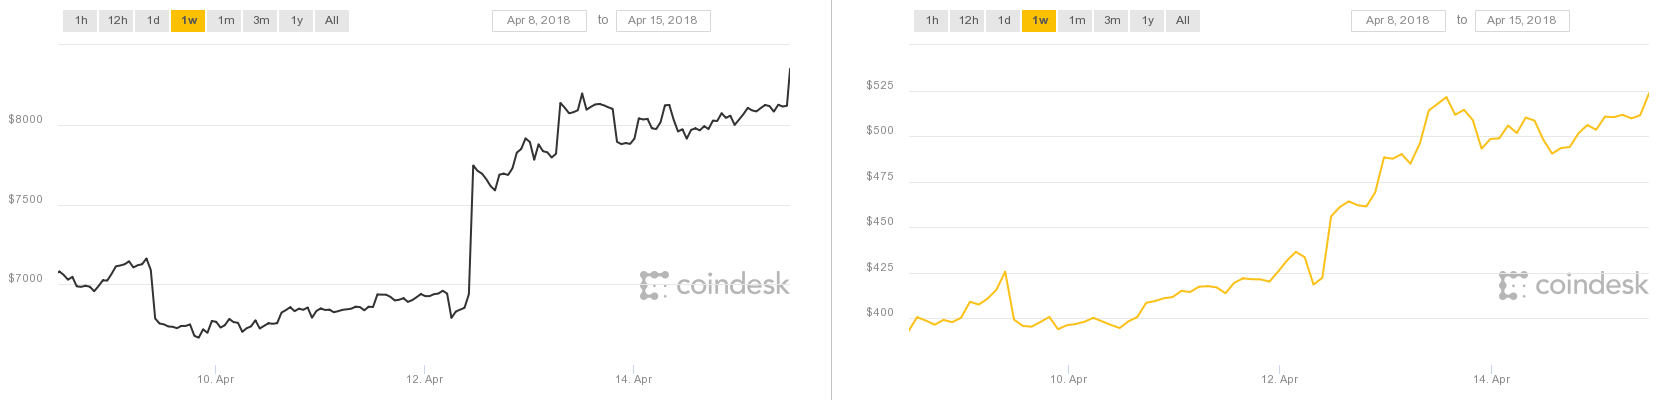
\includegraphics[width=\textwidth, keepaspectratio]{pricecharts/btceth1W.png}
    \caption{BTC and ETH Prices, Apr 8 - 15 2018 \cite{coindeskprices}}
    \label{prices1w}
\end{figure}    

While one could consider this purely coincidence, with a week arguably not being long enough to decipher any relationships between the two, the same can also been seen for a longer period of three months. Consider \textit{Figure \ref{prices3m}} below.

\newpage

\begin{figure}[h]
    \centering
    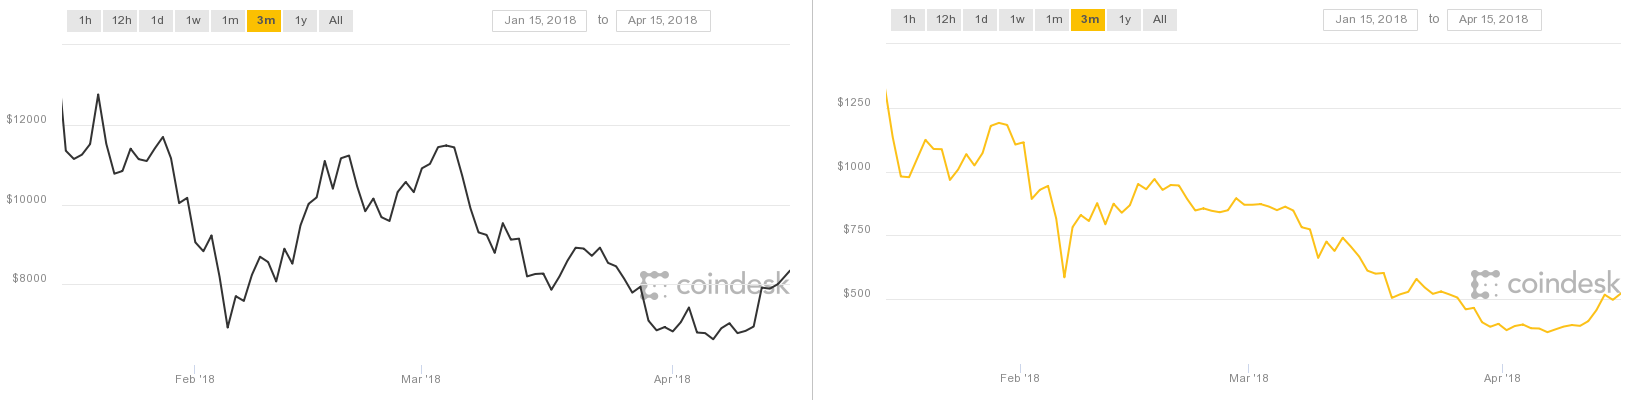
\includegraphics[width=\textwidth, keepaspectratio]{pricecharts/btceth3M.png}
    \caption{BTC and ETH Prices, Jan 15 - Apr 15 2018 \cite{coindeskprices}}
    \label{prices3m}
\end{figure}

In both instances, the prices of both Bitcoin and Ethereum follow roughly the same path. Bitcoin prices can be seen to be much more volatile, rising and falling more severely and in shorter spaces of time than Ethereum prices. For example, one should consider the sharp rise in price of Bitcoin shortly after April 12, 2018 against the slightly more dulled rise of Ethereum. This can also be observed in the rise and fall of the prices from Febrary to March 2018; the price of Bitcoin is seen to be more erratic, detailing many sudden increases and decreases. Ethereum follows the same general path with less sharp changes, implying that Bitcoin does lead to increased buying or selling of Ethereum. 
  
\subsubsection{Hyperbole Across the Media}
As introduced above, media content can often play a large role in the changing of currency prices. Of course, it is hard to effectively quantify the effect of social media coverage by simply observing prices on a graph.

In a very recent article, Mai et al found that social media in particular can be a relatively accurate predictor of future Bitcoin prices \cite{socmedimpact}. Focusing on one of the more popular forums for discussing Bitcoin, \textcolor{NavyBlue}{\url{bitcointalk.org}}, Mai et al concentrated on forum posts over three years, from 1 January 2012 to 31 December 2014. Data was also obtained from \textcolor{NavyBlue}{\url{Twitter.com}}, in the form of tweets containing the \textcolor{NavyBlue}{\href{https://twitter.com/hashtag/bitcoin?lang=en}{\#Bitcoin}} hashtag.

By using natural language processing to determine the number of positive or negative posts, Mai et al carried out tests on the obtained data through the use of vector error correction models to detect any interdependencies between pricing and social media coverage. Based on extensive testing as outlined in \cite{socmedimpact}, Mai et al found that social media activity is in fact at least a partial indicator or future Bitcoin prices.

Concluding their findings, Mai et al also highlight the issue of silent majority, vocal minority; in that most social media uses simply observe content as opposed to actively discussing the content. While this of course will skew results, the authors found this issue to be less common in the specified forum as opposed to Twitter. The group therefore concluded based on tests that any sentiments expressed on a forum have a bigger bearing on Bitcoin prices than those expressed on Twitter.

\subsection{The Bitcoin Bubble}
A bubble, defined as \textit{"a state of booming economic activity that often ends in a sudden collapse"} \cite{bubbledef}, is a term commonly used in conversations across a variety of finance-related conversations. Often referring to a very lucrative or advantageous period of time, these occurrences rarely last long, often "popping" suddenly as a physical bubble would.

\subsubsection{Historic Similarities}
The world has seen many bubbles end badly in the last 20 years, most notably "The Great Recession" which began in late 2007 \cite{greatrecession}. Prior to this downturn, the economy of the developed world had enjoyed great success financially, with financial institutions fuelling this by offering increased levels of loans and mortgages. 

While there are ongoing arguments as to whether Bitcoin is a bubble or not, and what the severity of a possible crash will be in the event that it is, it is hard to definitively agree with one argument or another. Any bubble in regards to Bitcoin would be brought on much differently to that of The Great Recession, and would likely run its course and recover differently to how the world economy recovered from The Great Recession. There are substantially more influences in the activity of the world economy than there are for any cryptocurrency activity, the prices of which are governed solely by demand.

One example of a historic bubble which has been likened to the popularity seen by Bitcoin is that of the "tulip mania" bubble experienced by the Netherlands in the 1600s. While the tulip mania bubble was not as disastrous or as widespread as is commonly believed, it did leave many merchants in debt. Similarly, if Bitcoin were to collapse tomorrow, only those who had invested would be affected and not the national or international economy. Unlike tulips however, Bitcoin does have core uses outside of simply existing; it can be used as a transferable asset, as well as a store of value \cite{tulipmania}. 
\subsubsection{The Future of Bitcoin}
Of course, with such a volatile asset as Bitcoin, it is hard to say if any major collapse will ever occur, or if prices would ever recover from such a collapse. Any possible collapse of Bitcoin could occur for a number of reasons, such as the advent of quantum computers capable of compromising the blockchain, or a simple sudden loss of faith in the resource.

The initial years of Bitcoin saw a relatively stable increase in prices, slowly climbing to just under \$1000 by the end of 2016 \cite{coindeskprices}. It is clear this growth in price was fuelled by a gradual, natural growth of Bitcoin's popularity, easily seen by exploring the popularity of the term in Google searches over time \cite{googletrendbtc}. For most of its life, Bitcoin had been a relatively unknown term, or at least certainly not understood by the majority. In 2017 however, the term began to gather momentum are prices surpassed the \$1000 mark, with prices rising exponentially for the duration of 2017. At Bitcoin's peak of \$19,661.63 on 17 December 2017 \cite{coindeskprices}, prices had risen by a staggering 1870\% in one single year. While there is no concrete calculation that can be done to determine what actually qualifies as a bubble, the sharp, almost irrational growth of prices would be difficult to refer to as anything other than a bubble. In keeping with the characteristics of every boom and bust cycle, Bitcoin suddenly plummeted to \$13,857.14 on 22 December 2017. In the months since, prices have continued to rise and fall toward an overall gradual decline, which could be interpreted as simply a correction of the ridiculous prices to prices that reflect more accurately the cryptocurrency's worth, as opposed to an actual crash. 

As very recently summarised well by Derousseau in \cite{airoutbubble}, factors such as increased interest by governments, the arrival of Bitcoin futures, and the growing number of alternative cryptocurrencies could all be leading factors in price declines. Bitcoin has now been banned by governments in a number of countries, which of course negatively affects the market as those countries' residents sell of their currency. Bitcoin futures, allowing investors to simply bet on whether Bitcoin prices will rise or fall, means that those interested in cryptocurrency no longer need to own that currency in order to profit from it, possibly leading to a decline in the market in future. Lastly, as more cryptocurrencies are added to the market, the market space for existing currencies reduces. While popularity of the bigger currencies may remain steady, the addition of newer varieties is likely to steal some of the spotlight from Bitcoin as people invest early with the hopes of these new currencies eventually reaching Bitcoin prices.

To conclude, the volatility of Bitcoin prices and cryptocurrency prices in general determines that one will likely never be able to accurately predict the price changes of these currencies. While Bitcoin itself may have gone through a bubble-like phase in 2017 and early 2018, its stabilisation is unlike that of a national economy after a financial crash. Perhaps Bitcoin will continue on a path similar to that of the last year, rising and falling but remaining in the order of thousands of dollars per coin. Perhaps interest and ultimately faith in Bitcoin will dwindle, resulting in the outright collapse of the currency. Nonetheless, it would be absolutely absurd to claim one or the other will definitely occur - we are simply going to have to observe these events as they happen.

\section{Deciphering Trends in Prices}
It is with this knowledge in mind that we progress to the applied aspect of this project. As examined above, there is no method to accurately predict the prices of any cryptocurrency. However, there are certainly trends in prices, which can be examined and attempted to be forecast using a variety of new technologies. 

Building on the information discussed in this and previous chapters, we will now examine the applied element of this project; a web application for displaying Bitcoin prices against the Euro and predicting future values of Bitcoin. 

It should be noted that while the web application was designed to be as easily understood as possible, it is still encouraged that the user has at least partly read and understood the preceding chapters of this dissertation.

\chapter{Currency Analyser Web Application}\label{applprojch}
In this chapter, we will examine all components of this project, theoretical and applied, by reflecting on the approach to the process from its inception to is concluding days. The research and development methodologies used throughout this project will be explained, including any aspects the team would have done differently in hindsight. The technologies behind the web application are explained, as well as any team decisions behind using them and any problems encountered during their integration into the project. The overall design of the finished system is then analysed, concluding with an evaluation of the system.

\section{Methodology}\label{secmethodology}
In this section, the way in which the project was planned, organised, managed and decisions made throughout its life cycle will be discussed. Initial research and decisions regarding the team's approach to this project will be examined, before detailing any differences in the way in which this project ultimately panned out.

\subsection{Preliminary Research and Project Commencement}\label{prelim}
The team had their first meeting in late September, shortly after specifications for the project and dissertation had been given. It was agreed that getting started as soon as possible was best, and an agreement was reached to decide on an idea and carry out some research before starting any of the applied aspects of the project. 

While the team had a number of basic possible concepts which would be suitable for the scope of a final year project, taking on a data analytics project in the form of analysing cryptocurrency was considered to be the most interesting. The team had also agreed that machine learning should be incorporated into the project if possible, and saw pursuing this idea as an opportunity to include some innovative machine learning technologies in an interesting and relevant way. It was decided that a web application containing graphs of currency prices and a future price prediction feature would be ideal for this purpose and to demonstrate all theoretical aspects of this project, which would be discussed in the dissertation.

Following this decision, the first meeting with the team's supervisor was organised, in which all ideas were discussed. It was agreed that a cryptocurrency data analytics project would be a suitable and interesting project, and the team were given advice as to what technologies should be considered for use. Taking this advice on board, the team began more detailed research.

\subsubsection{Research Methodology}\label{secresearchmeth}
As all team members had some previous experience with cryptocurrency, it was agreed that major preliminary research into the concept was not a requirement. The team did some light reading of the latest news items relating to cryptocurrency and moved on to researching a list of technologies, examining which would be best to include in the applied project.

\textbf{\textit{Database of Prices:}} Based on the team's collective experiences from the previous academic year, it was first agreed that \textit{Python 3} would be ideal for obtaining data. The team carried out some quick searching online and found there to be numerous free cryptocurrency APIs (\textit{Application Programming Interfaces}) available, all of which stored vast amounts of records for prices of cryptocurrency against a variety of traditional currencies for increments of time, usually every minute. The team concluded this was often enough for a web application which does not deal with trading and therefore does not need to be accurate. After refreshing collective knowledge of MongoDB documentation \cite{mdbdocs}, the team agreed on using a MongoDB database to save data into from an API via a Python 3 script.

\textbf{\textit{Web Application Back-End:}} Having decided the details of the project's database system, the team began discussing the back-end of the application. Once again, previous experiences encouraged the use of Python 3 and the Flask Framework. All team members had enjoyed using this combination for previous web application projects, and felt it would simply make sense to do so again.

\textbf{\textit{Web Application Front-End:}} Based on the advice of the team's supervisor, research on \textit{Vue.js} \cite{vuejs} and \textit{D3.js} \cite{d3js} was carried out. It appeared this combination would work well for creating a web application with simple yet intuitive design, as well as creating striking visual representations of our data.

\textbf{\textit{Web Application Hosting:}} During prelimary research, the team considered both Microsoft Azure \cite{azure} and Heroku \cite{heroku} for deployment of the final application. Having deliberated over the technologies for some time, the team considered using Microsoft Azure due to previous experience and its vast quantity of features, all of which could be confidently relied on. However, it was noted that this was not a definite decision at the time, and the team were still open to the possibility of using Heroku if it were more suitable when the time came to deploy the application.

\textbf{\textit{Containerisation:}} Having heard about the benefits of containerisation, the team researched Docker \cite{docker}, a leading platform in containerisation. Containerisation, put simply, is the packaging of applications \textit{with} all relevant libraries and dependencies. This feature eliminates issues when trialling applications on different machines which may arise due to conflicts in installed software and the software the application was initially built with. While this was not a crucial element to the project, it would be convenient to implement should any related problems arise.

\textbf{\textit{Machine Learning:}} With regards to attempting to decipher trends in prices, the team's supervisor recommended the use of TensorFlow \cite{tensorflow}. Having been using this machine learning framework in class for some time at this point, the team were familiar with the framework and had been using the technology with Python 3. It was agreed that this combination should be used, as it would fit in well with the overall project architecture.

\subsubsection{Initial Expected Architecture}
Based on the research described above, the architecture depicted in \textit{Figure \ref{initarchitecture}} was decided upon. Of course, no aspect of this architecture was a concrete decision as the team felt it necessary to allow for discovery of new, possibly more suitable technologies.

\newpage

\begin{figure}[h]
    \centering
    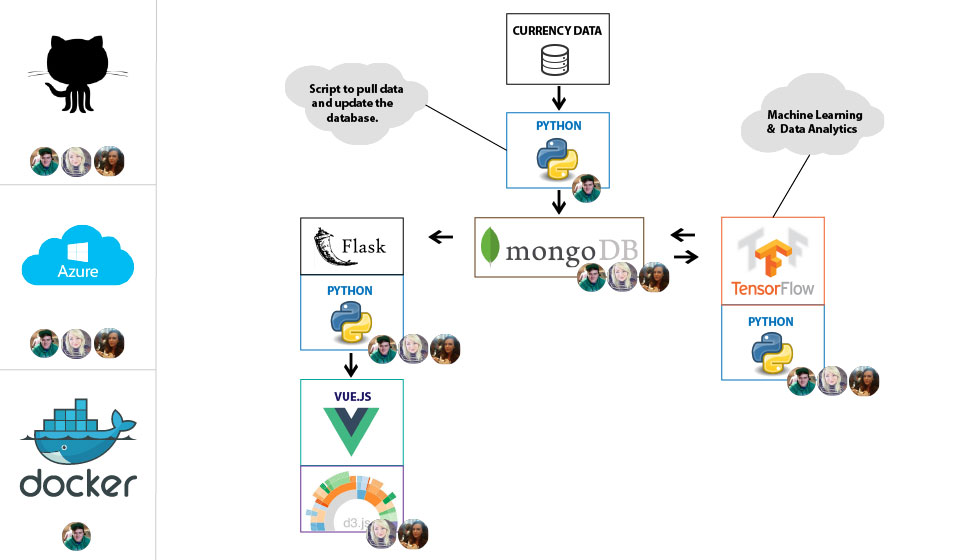
\includegraphics[width=0.9\textwidth, keepaspectratio]{img/Architecture.jpg}
    \caption{Planned Architecture, \textit{October 2017}}
    \label{initarchitecture}
\end{figure}

\subsubsection{Agile Development}
Having learnt about the various approaches to software development in previous academic years, the team felt that the \textit{Agile Methodology} \cite{agilemani} was the best to follow. In \cite{agileieee}, Highsmith et al highlighted the attractiveness of the agile approach, stating that working code and a team who work together effectively are the two main concepts stressed in agile methods \cite{agileieee}; working code proves to both developers and clients exactly what has been done, and an effective team can achieve cost savings as well as flexibility. Regular interaction between team members and the closeness of a team are also fundamental to agile methods, further pointed out by Highsmith in \cite{agileieee}. The team agreed this was the ideal methodology to follow, as regular communication and a stable, consistent timeline of work were strongly desired. 

Agile approaches often include the division of work into short periods of time called sprints, often a two to six weeks in length. At the beginning of each sprint, a goal for the end of the sprint is defined, such as a particular component of the project to be working, or some element to have been tested extensively. It was agreed that the inclusion of four week sprints in this project's life cycle would further help the team to keep on top of the project workload, providing a definitive timeline of progress.

\subsubsection{Version Control}
Having used free online version control software GitHub for a number of years, the team decided it would be ideal for keeping track of source code throughout this project. One particularly useful feature of GitHub is branches, allowing users to push to a given repository without necessarily affecting the original master branch. The team intended to have a branch for each member's work, a branch for developing (where individual work would be tied together), a branch for testing, a branch for machine learning, and a branch for dissertation work. Workload was divided between the team members as follows:

\begin{itemize}
    \item Tara O'Kelly: Front-End Development, including visualising currency data on a graph.
    \item Johnny Glynn: Back-End Development, including obtaining and saving currency data.
    \item Rebecca Kane: Dissertation, including relevant research.
\end{itemize}

It was decided that it would be best if the team worked collectively on any machine learning elements after the work specified above was complete, and thus didn't initially allocate it to any one member. 

It was acknowledged that GitHub's \textit{Issues} feature would come in very useful for keeping track of any problems. The team planned to use this to organise both technical code-related issues and issues related to the dissertation, such as information being required from one member or another on a particular subject or technology.

GitHub's \textit{Projects} resource would also add to the overall organisation of the project. \textit{Projects} are very similar to to-do lists and can be used in conjunction with Issues, allowing to-do items to be assigned to certain members. GitHub allows the creation of multiple \textit{Projects}, meaning one could be created for each major component of this project, such as Dissertation or Machine Learning.

\subsubsection{Testing}
It was agreed by the team that in keeping with the metrics discussed in \textit{\ref{metrics}: Metrics for Success or Failure}, testing should be user driven for the most part. Based on the metrics outlined in the aforementioned section, the team decided on the following tests related to each metric: 

\begin{itemize}
    \item\textit{Metric One - Easily understood, cohesive dissertation}: In order to test whether the team had succeeded in providing a clear and comprehensive examination of cryptocurrency in this dissertation, the team agreed it was best to ask those who had little or no understanding of cryptocurrency to read Chapters \textit{\ref{understandingcryptocurrencych}: Understanding Cryptocurrency} and \textit{\ref{predictingpricesch}: Predicting the Prices of Cryptocurrency}. It was decided that those who read the chapters would be asked to rate how well they understood the content on a scale of one to five, with one being no understanding and five being perfectly understood. The team agreed a test sample size of five or six people would suffice.
    \item\textit{Metric Two - Simple Web Application}: Again, it was decided that in order to test the simplicity of the web application, it would be best to ask those who had little or no knowledge of cryptocurrency. Similar to the above, five users would be asked to use the web application for a brief period of time and provide feedback on their opinions of its usability, using the same scale as above.
    \item\textit{Metric Three - Future Cryptocurrency Price Estimates}: In order to test the accuracy of the web application's predictions, it was agreed that the predictions should be tested over a period of one week, or seven predictions. Due to TensorFlow's training and testing facilities, this test could be carried out in one sitting. The TensorFlow model would be trained, and subsequently shown seven unseen prices, and asked to predict the new price. For example, the model can be shown a price from 11 December 2017 and asked to predict the price for the following day, which can then be compared against the actual data from 12 December 2017.
    \item\textit{Metric Four - Teamwork}: Of course, teamwork is not something which can be measured in a definitive way. It was determined that in order to measure the success of this, the team would simply reflect at the conclusion of this project on how issues were resolved, and if relationships were affected by any disagreements. 
\end{itemize}

\subsubsection{Supervisor Meetings}
During the first meeting with the team's supervisor, it was discussed what the frequency of supervisory meetings should be. The collective feeling was that a weekly meeting would be too often, as some weeks would naturally allow for more or less work to be done than others. It was determined that it was best not to have meetings if a substantial amount of work had not been done, and it was concluded that meetings would be best if only had when warranted, ideally every few weeks.

\subsection{Issues Encountered During the Development Process}\label{issuesencountered}
While the team initially had great intentions and did begin work on this project as soon as requirements were available, numerous issues ultimately surfaced.

\subsubsection{Interfering Factors}
Of course, at certain stress points throughout the academic year, work on this project was postponed due to upcoming exams or deadlines related to the team's other projects. As the first semester of this year involved more modules and therefore more work than the second semester, the collective decision was made by the team to put other projects first from late November 2018 through to early January 2018, when the second semester began. However, significant progress was made by the team between September and the end of November and this decision was believed to not have seriously jeopardised the progress of this project. A supervisory meeting was arranged in late November to discuss the work achieved thus far, and again in early January to discuss the direction of the project from that point. After regular contact with the team's supervisor, work proceeded again from mid January onwards.

\subsubsection{Communication Issues}
While communication was not an issue in the first semester of this year, it quickly became a problem as one team member unfortunately became ill in late January 2018, and remained so for the rest of the duration of the project. Contrary to what Agile development encourages, the team began to rely on messages, emails and occasional phone calls in order to keep in contact with the absent member. This ultimately led to a strain on development, as it grew more and more difficult to express ideas, plan for subsequent work through messages and calls. As the Agile Manifesto states, \textit{"The most efficient and effective method of conveying information to and within a development team is face-to-face conversation"} \cite{agilemani}. The team fully supports this statement, as there was no comparison between discussing components of the project through practical examples in person, and trying to do the same simply over the phone. There were also a number of occasions where a meeting was agreed for a certain day and time, only to result in two members being present due to lack of communication.

These communication issues ultimately delayed development, as other team members had to wait on the absent member to publish work on GitHub or reply to messages, as opposed simply seeing each member's work in person, or talking face to face and having an immediate reply. 

\subsubsection{Lack of Working Code}
As mentioned in the previous section, one team member had become ill and was absent from late January onwards. The two remaining team members continued to work on research based elements for some time, as they required work from the ill member in order to progress properly with their own work. While we acknowledge that some work could have been done by the remaining members by assuming the work of the absent member had been done in a certain manner, any progress made by the remaining members would ultimately have had to have been altered to suit the absent member's work. This method likely would have resulted in integration problems closer to the deadline, and thus it was decided that we would wait for the absent member to publish their code on GitHub.

While the absent member reassured remaining members that work was being done, there had been a lack of published code on their behalf since the previous semester. Nearing the end of the project, the remaining members continued to request that they see working code on the basis of being unable to spend any more time not moving forward in development. 

\subsubsection{Resolution of Problems}
On the basis of the issues discussed above, two members of the team brought their concerns to the project supervisor to look for advice. The options of continuing along the same track with all members contributing to the one project, or a division of the group to work on two separate projects were presented to the team. A discussion was held between all three team members, and it was mutually agreed on 9 April 2018 that the option to work as two separate teams from then on was best for all members. Keeping in mind the teamwork objectives outlined in \textit{\ref{objectives}: Objectives} and \textit{\ref{metrics}: Metrics for Success or Failure}, the team agreed to not let any of these issues affect their friendships, and have succeeded in doing so thus far.

\subsubsection{Development Following Group Partition}
As there was little time left after the decision to separate into two groups, development in the last week of the project became somewhat erratic, following aspects of Extreme Programming development methodologies. The team could not afford to put large quantities of time into planning, and thus decided to only use a few hours to plan for what needed to be completed in the week ahead. 

\textbf{\textit{Extreme Programming:}} Based on the fundamentals of the Extreme Programming methodology, outlined by Wells in \cite{xp}, this methodology is successful partly due to its encouragement of developers adapting to change, sometimes late in the development life cycle. The loss of one team member could be considered difficult to adapt to so late in this project's life cycle, but the team decided to follow the principles of Extreme Programming closely in order to overcome this. The team decided to self-organise around the problem to solve it as quickly as possible \cite{xp} and began reallocating tasks based on their importance. Once tasks had been outlined the team kept Wells' summary of a successful Extreme Programming project in mind - \textit{communication, simplicity, feedback, respect, and courage}. Over the final week of the project, the team kept in near constant contact with each other, also regularly discussing various facets of the project with their fellow students. Of course, at such a late stage the design of any further implementations must be as simple and clean as possible, a concept the team strived towards. Rather than test numerous implementations and methods, the team decided it best to research possible solutions to any problems, before implementing them. Ultimately, this saved much time, as a chosen solution was subsequently well understood and highly likely to work as expected. Finally, in keeping with initial objectives for this project, the team aspired to continuously be respectful in this time of high stress, while being courageous and trusting in their own decisions.

To conclude, the final week of this project was of course very demanding and stressful. One may have expected any work produced in this time frame to be cluttered, thrown together with haste in an attempt to meet deadlines. Fortunately, the quality of work by the team actually improved due to the crucial planning necessary in order to produce a large amount of work in such a short period of time.
\section{Underlying Technologies}\label{sectechnologies}

\subsection{Python 3}
Python is a high-level, easy to read programming language, ideal for programmers with any level of skill. Python has become one of the most widely used programming languages, certainly due mostly to its simple yet powerful design. Unlike languages such as \textit{Java} and \textit{C}, Python syntax is relatively uncomplicated and thus not as daunting as more traditional languages. This theme carries across into Python documentation \cite{pythondocs}, which remains simple and arguably easier to understand than, for example, Java documentation. 

For the purposes of this project, the Anaconda distribution \cite{anahome} of Python 3 was used, as it is aimed at data science and machine learning applications. Anaconda's virtual environment manager, Anaconda Navigator, is included with the open source distribution and makes installation and updating of packages a much simpler process. There are a large number of external libraries available in the Anaconda distribution of Python 3, including some powerful data science packages like Scikit-learn, TensorFlow, and SciPy. It was for these reasons, as well as past experience with Python 3, that the team chose to work with this particular distribution.

\subsection{The Flask Microframework}
The Flask microframework \cite{flaskhome} is designed for building simple web applications with a Python back-end. By using the Anaconda distribution, Flask can be installed simply through Anaconda Navigator, and all Flask applications can be run on any computer and accessed via opening a browser at \url{http://127.0.0.1:5000/}. The back-end of a Flask application looks very similar to a standard Python file, with added \mintinline{python}{@app.route()} decorators to handle what happens at specific URLs. For example, \mintinline{python}{@app.route("/")} defines the home page of any web application, which in most cases simply loads the specified html file when the URL is called in the front-end. In short, the Flask microframework allows users to create web applications with a Python back-end quickly and easily.

\subsection{Redis}
While MongoDB had initially been intended for use as the store for currency data, research into Redis was carried out based on advice from the team supervisor. Redis, meaning \textit{REmote DIctionary Server}, is an open source in-memory data store which supports many different data types \cite{redishome}. The use of in-memory storage as opposed to disk storage offers a number of advantages, mainly making retrieval of data in Redis extremely fast, capable of performing roughly 110,000 \mintinline{MySQL}{SET} operations or 81,000 \mintinline{MySQL}{GET} operations per second \cite{redistut}. While Redis can be used for multiple purposes, such as caching or message queues, its main purpose in this application was the storage of short-lived currency data.

\subsubsection{Forex-Python}
The Redis store of currency data within this project is updated using a Python script, which obtains the data using the \textcolor{NavyBlue}{\href{https://pypi.python.org/pypi/forex-python}{forex-python}} library \cite{forexpy}. This library contains prices for most traditional currencies, as well as prices for Bitcoin obtained through CoinDesk's \textcolor{NavyBlue}{\href{https://www.coindesk.com/api/}{Bitcoin Price Index API}} \cite{bpiapi}.

\subsection{MongoDB}
MongoDB is an open-source document-based database \cite{mdbdocs}. As mentioned in the above section, MongoDB was initially considered for the storage of currency data, subsequently replaced with Redis. However, the machine learning data and predicted prices of Bitcoin also needed to be stored somewhere. While Redis is suitable for short-lived currency data, it would not be suitable for storing any data related to the machine learning element of this project. It was decided by the team that due to previous knowledge of MongoDB, it would make sense to use it in this respect.

Within a separate Python script, data is obtained from the \textcolor{NavyBlue}{\href{https://pypi.python.org/pypi/forex-python}{forex-python}} library and saved into a MongoDB document. As the machine learning model does not need to be retrained regularly, this is done at a much lesser frequency than that of the Redis script.

\subsection{Vue.js}
Vue.js is a JavaScript framework for building user interfaces, designed to be capable of integration into a project at any stage. Despite the team having no experience with Vue.js, the technology was adopted following advice from the team's supervisor and some intensive research and tutorial-based learning. While Vue.js was initially difficult to adapt to, the wide variety of tutorials and documentation available online greatly helped. The team did briefly consider changing to an alternative framework, but determined it was best to continue with Vue.js due to the time invested in learning. Ultimately, Vue.js proved to be a powerful tool; one the team would be comfortable working with again in the future. 

\subsubsection{Chart.js}
The team had initially intended to use D3.js to handle the representation of currency data through graphs, and spent a short period of time attempting to develop the application with this technology. After some difficulty with integration of D3.js in the initial weeks of development, the team had discussed the technology with fellow students who had also found D3.js difficult to incorporate into projects. Based on recommendations by fellow students, the team researched a similar technology called Chart.js.

Chart.js \cite{chartjs} allows developers to display data in a number of differently formatted graphs, all of which are capable of animation and customisation. Using the simple HTML5 \mintinline{html}{<canvas> } tag, Chart.js was much easier to adapt to than D3.js. Following brief research and some online tutorials, the team opted for the simplicity of Chart.js. Considering the graphs in this project did not need to do anything extraordinary, Chart.js was perfectly suited to this application.

\subsection{TensorFlow}
TensorFlow is an open source framework, designed to allow high performance numerical computation for machine learning purposes \cite{tensorflow}. The software can be used with a number of languages such as C and C++, with the most popular and well-documented language being Python. 

TensorFlow is based upon data flow graphs. Simply put, data flow graphs detail an input, some operations often on multiple levels, and an output. With regards to TensorFlow, each node in a graph represents a mathematical equation to be performed on the given edges which contain data (often multidimensional data arrays, described as tensors) which flow between them.

TensorFlow can be used in many applications, such as type prediction, value prediction, and image recognition; this application of TensorFlow within this project concerns value prediction. Data is loaded in, manipulated into the correct format to work with a specific model, and fed to that model. The model is first trained using historical data, in this case previous prices of Bitcoin, until it computes the correlation between actual and predicted values. Once trained, the model can be given unseen data to be tested. TensorFlow was deemed the most suitable technology for the machine learning aspect of this project, due to the the team's previous experience of the technology and its extensive documentation and tutorials available online.

\subsection{Heroku}
Having initially expected to use Microsoft Azure for application deployment, when it came time to begin thinking about deploying the application it became obvious that this technology was excessive for this instance. As mentioned previously, Microsoft Azure offers an extensive range of services, and thus can be quite complex to use even for the most basic of applications. The team had also considered Heroku in the beginning and having since gained more experience of the technology through other projects, decided it was the best option for this project. 

Heroku is an open source cloud application platform, providing extensive documentation for many facets of the deployment process and life cycle \cite{herdep}. Heroku is arguably much easier to use than Microsoft Azure, allowing a developer to create and deploy an application from scratch in a very small amount of time. Heroku also allows applications to be deployed using Git, a tool the team were very familiar with due to extensive previous experience of GitHub. It was for the ease of deployment and comprehensive, easy to follow documentation that the team ultimately decided to use Heroku when deploying this application.
\section{System Design}\label{secdesign}

Throughout the development life cycle there were a number of changes regarding technologies and overall design of the web application. Having initially intended to follow the architecture detailed in \textit{Figure \ref{initarchitecture}}, a number of problems and events ultimately led to some changes.

The restructuring of this application was not major but did greatly benefit the project, seeing the addition of new technologies and removal of those that were deemed unnecessary. In this section, the overall design of the web application will be explained under the following headings; \textit{Web Application}, \textit{Currency Data}, and \textit{Machine Learning}.

\subsection{Web Application}

Flask Blueprints \cite{flaskblueprints} are adopted in this web application to organise and separate distinct components or modules, in this case the client and the \textit{Application Programming Interface} or API. Blueprints define a collection of behaviours, views, templates, and static files which can be then used anywhere in the application. Although this project does not intend to take advantage of the reusability of blueprint modules, it will benefit from the elegant architectural structure that can be achieved with them. 

The application consists of two separate blueprints registered to the following URL sub-domains: \mintinline{python}{""} and \mintinline{python}{"/api"}. The client has the responsibility of serving the HTML files to the user and can be accessed as such: \textcolor{NavyBlue}{\url{https://currencyanalyser.herokuapp.com/}}. The client has one route, \mintinline{python}{"/"}, that returns the single page web application, in the form of the index.html file that links the built and minified Vue.js code via a script tag. The single page web application consists of the following pages:

\begin{itemize}
    \item \textit{Home:} This is the root page, containing the application title. Page URL: \textcolor{NavyBlue}{\url{https://currencyanalyser.herokuapp.com/}}
    \item \textit{Dashboard:} This is the main page of the application, displaying a collection of cards containing prices and rates of various currencies, along with machine learning predictions of Bitcoin prices. Cards containing graphs were originally going to be rendered using the D3.js library, a fantastic data-driven approach to Document Object Model manipulation. However, D3.js was unnecessarily sophisticated for its use being solely to create dynamic graphs. Chart.js is a simple but powerful data visualisation library, that serves the purposes of this project perfectly. Page URL: \textcolor{NavyBlue}{\url{https://currencyanalyser.herokuapp.com/#/dashboard}}
    \item \textit{About:} This simple "About" page contains details relating to the team, context of the project and contact details. Page URL:\\ \textcolor{NavyBlue}{\url{https://currencyanalyser.herokuapp.com/#/about}}
    \item \textit{Error:} This is a standard error page which displays when any URL containing a domain which is not mentioned above is queried. Page URL: \textcolor{NavyBlue}{\url{https://currencyanalyser.herokuapp.com/#/some\_invalid\_url}}.
\end{itemize}

The project's API has the responsibility of returning machine learning and currency data and can be accessed via \textcolor{NavyBlue}{\url{https://currencyanalyser.herokuapp.com/api/}}. The API blueprint utilises the Flask-RESTful extension, adhering to the standard architectural design for web services and web APIs.

\subsection{Currency Data}
The project's API populates data to be returned through the use of background workers, which are used to pull data at scheduled intervals of $n$ seconds. These workers also pull data of $n$ days to train the machine learning model with the previous days result, and to predict the end price for the current day. Initially, the API was to act as the database handler or \textit{DAO (Data Access Object)}, controlling and encapsulating actual communications to MongoDB. The scripts would publish the new values and the API listener threads would handle the data received. 

However, during the implementation of this concept for handling data, we came upon the realisation that the API would be dealing unnecessarily with MongoDB. The web application only deals with the most recent data, and thus can be optimised by pre-formatting any data to suit the web application's requirements. The data from the API is requested and refreshed by the web application constantly for the most recent currency data. Consequentially, it would be cumbersome to query the MongoDB database and reformat the query result with every request. The scripts were already communicating with the API via Redis, thus it seemed optimal that the scripts handle MongoDB and use Redis solely to share the most recent data with the API. This would subsequently simplify the code and reduce the dependencies the scripts have on one another, e.g. the worker relies on the web application to save the data published, or the worker needs to be ran to allow a clean shutdown of the web application. The web application's Heroku CPU allocation is no longer competing with listener threads, and the management of MongoDB will be abstracted from the API rather than delegated to it. 

Furthermore, as the machine learning implementation developed we realised it would no longer require the live currency data, meaning it was no longer necessary to save real time currency data to the MongoDB database. Now this data will solely be used for live currency data displayed on web application.

\begin{figure}[h]
    \centering
    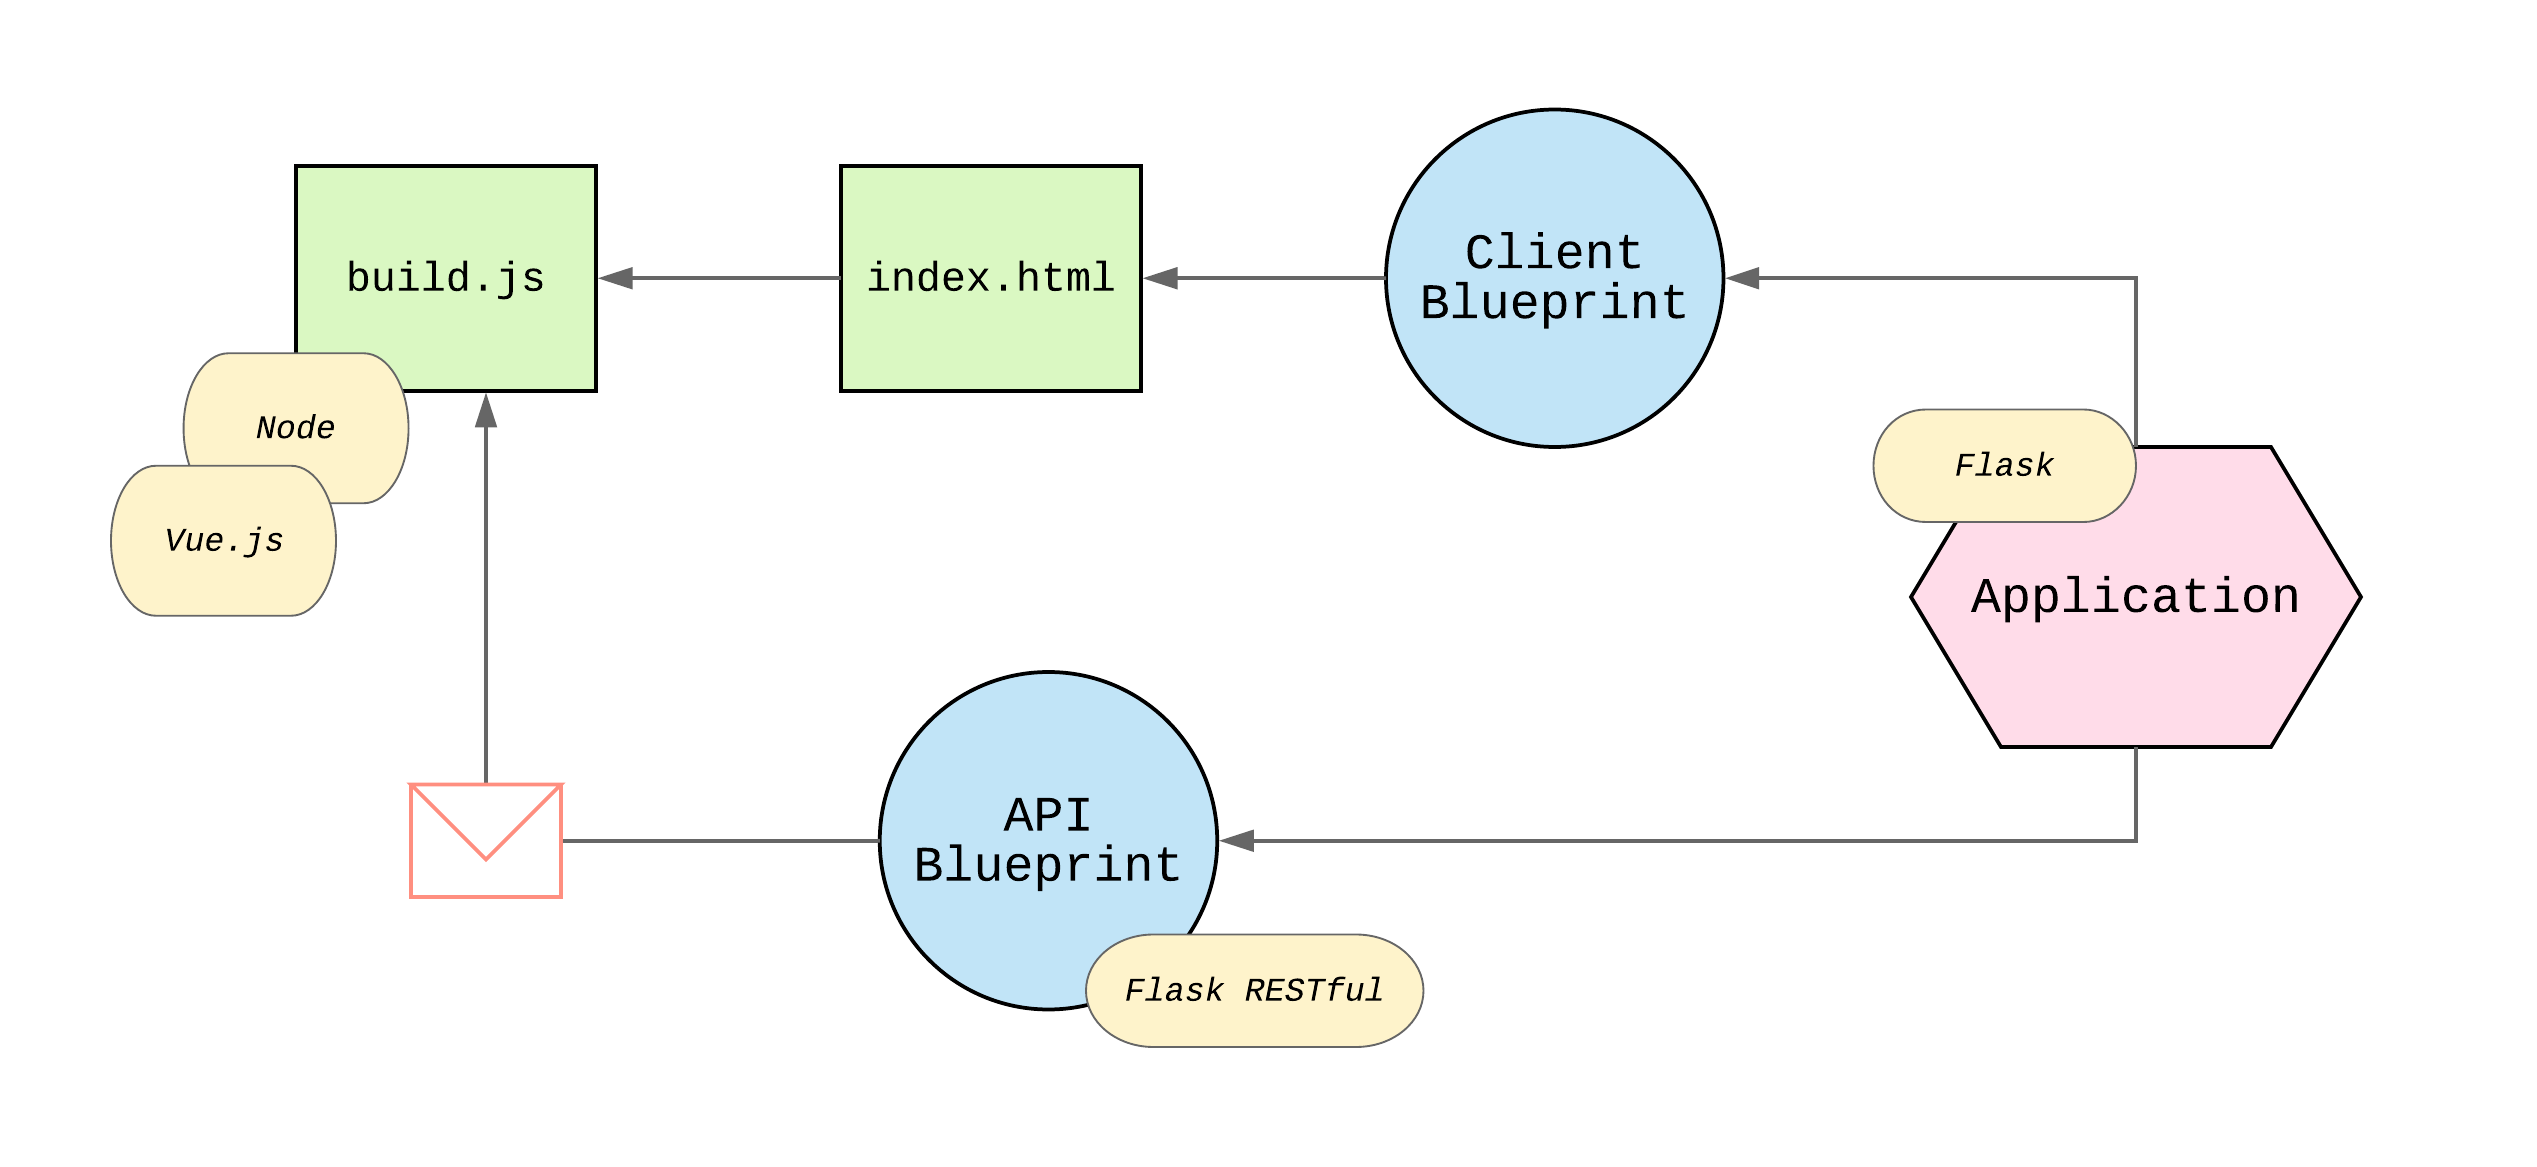
\includegraphics[width=0.9\textwidth, keepaspectratio]{img/techuml.png}
    \caption{Diagram of Application Design, \textit{April 2018}}
    \label{techuml}
\end{figure}

\subsection{Machine Learning}
The machine learning element of this application was built using Python 3 and TensorFlow. Machine learning is the use of statistics and computation in order to give systems the ability to "learn" and improve from past experience without being explicitly programmed to do so. Artificial neural networks, inspired by the biological networks within our brains, is the particular strain of machine learning which is used within this project.

The \textit{Long Short Term Memory} or LSTM algorithm, an efficient gradient-based model introduced by Hochreiter and Schmidhuber in 1997 \cite{lstm}, was used in the building of the neural network model for this system. \textit{Recurrent Neural Networks} attempt to address memory issues in traditional neural networks by adding loops within them, allowing information to persist \cite{colah}. A reasonable analogy, is to envision recurrent neural network as numerous copies of the same network, each passing a message to a parent. This chain-like nature resembles the behaviour of sequences and lists, making them naturally suited to the architecture of a neural network. 

Unfortunately, recurrent neural networks are burdened with the problem of handling long-term dependencies. As the neural network grows, gaps between past relevant data grows, and the recurrent neural network model becomes unable to learn to connect the information. In theory, recurrent neural networks are absolutely capable of handling this issue. In fact, some are. Long Short Term Memory is an extension or type of recurrent neural network that is capable, being very efficient on a large variety of problems including timeline data \cite{dashee}, and is now widely used to solve these problems. LSTM models have an additional loop learning what data to forget and what data to remember; they still have the aforementioned chain like structure, but with four different layers communicating in a certain way.


\subsubsection{Final Architecture}

In conclusion, the final architecture indeed differs somewhat from that which was originally planned. A diagram of the complete final architecture for the system is detailed below.
\\
\\
\\
\begin{figure}[h]
    \centering
    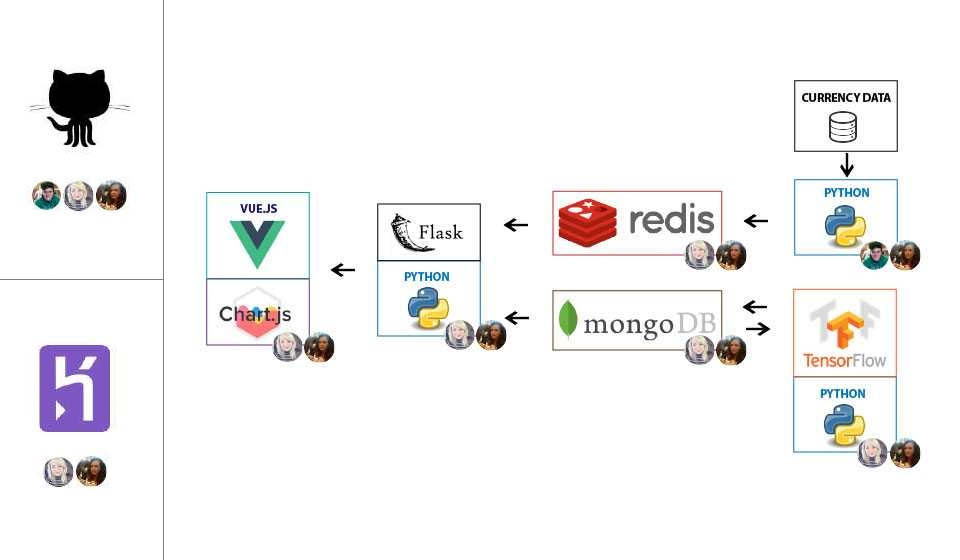
\includegraphics[width=0.9\textwidth, keepaspectratio]{img/newarchitecture.jpg}
    \caption{Final Architecture, \textit{April 2018}}
    \label{finalarchitecture}
\end{figure}
\section{System Evaluation}\label{seceval}
Reflecting on the objectives discussed in \textit{\ref{objectives}: Project Objectives}, the following is a condensed initial list of objectives for both the dissertation and applied aspects this project:\\

\textit{\textbf{Dissertation Objectives:}}
\begin{enumerate}
    \item Introduce the concept of the project.
    \item Provide the reader with a rounded understanding of cryptocurrencies.
    \item Explain to the reader how volatile cryptocurrency prices can be.
    \item Describe in detail the applied aspect of this project.
\end{enumerate}

\textit{\textbf{Applied Project Objectives:}}
\begin{enumerate}
    \item Create a simple web application which is easy to use and clear to understand.
    \item Deliver cryptocurrency prices to the user.
    \item Provide an educated guess as to future changes in prices.
    \item Work closely with the given learning outcomes for this project.
    \item Conduct work as a team, in a professional manner akin to what is expected in industry.
\end{enumerate}

\subsection{Testing}
Based on the objectives outlined above, the following tests were carried out to gain an insight as to the success and robustness of this application.

\subsubsection{Usability Testing}
Undoubtedly, a large portion of this project as whole surrounds explaining to the reader the fundamentals of cryptocurrency. The goals which cannot be quantified were considered to be all \textit{Dissertation Objectives}, and \textit{Objective 1} in the \textit{Applied Project Objectives} list. In order to measure the success of these goals, it was decided that the best was to do so was to ask others with varying levels of knowledge to read one or many chapters and briefly use the web application, and to gather feedback from them.

We created a survey through Google Forms, and sent its \textcolor{NavyBlue}{\href{https://docs.google.com/forms/d/e/1FAIpQLSfZQVFLgzG6dHy9U46xHPHuvzhitVnsvZaT1FXDjL-pFlgQTg/viewform?usp=sf_link}{link}} to those who had kindly offered to read this dissertation. All information other than the number of chapters read was on a scale of one to five.

The form asked participants five questions; their initial level of knowledge of cryptocurrency, which dissertation chapters they had read, how easy they felt terminology was to understand, how much the reading had improved their knowledge of cryptocurrencies, and how easy they felt the corresponding web application was to use. Identity remained anonymous, as it was deemed not required for the purpose of the survey. The link was only sent to those who had agreed to participate, and thus the form's results would not be skewed by anyone who had not participated.

A summary of the results is detailed in \textit{Figure \ref{surres}} below.

\begin{figure}[h]
    \centering
    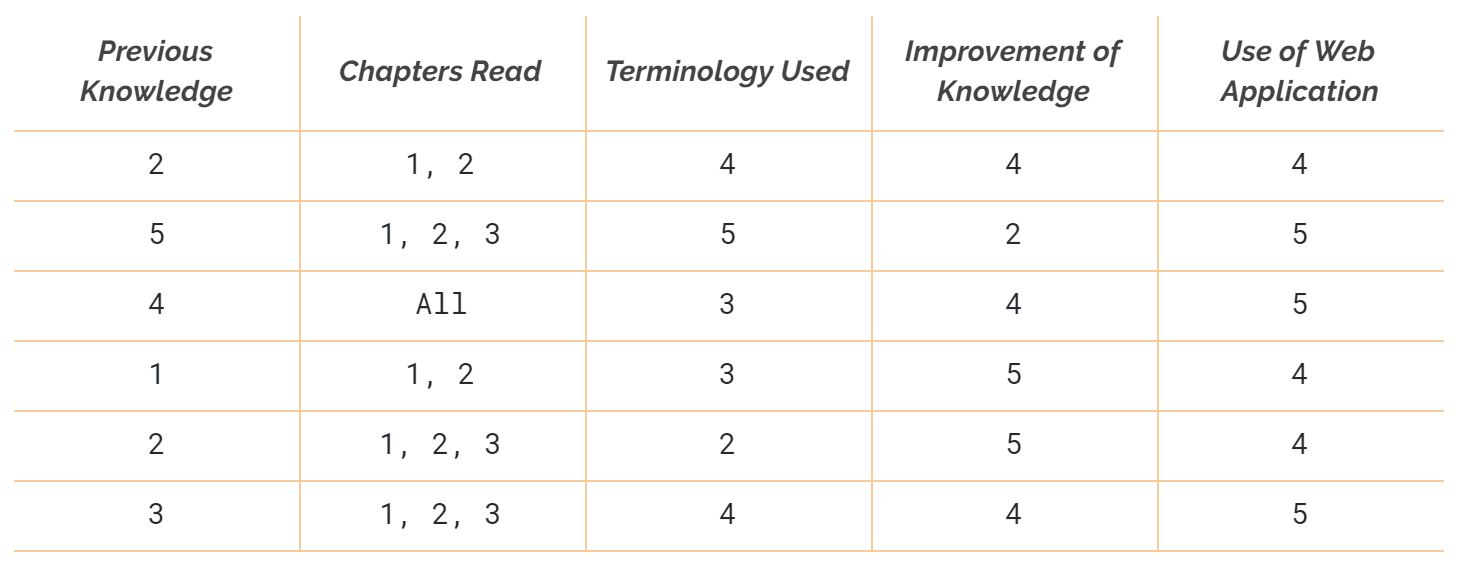
\includegraphics[width=0.9\textwidth, keepaspectratio]{img/testres.JPG}
    \caption{Survey Results \textit{April 2018}}
    \label{surres}
\end{figure}

Based on these results, we can conclude that while those with expert levels of initial knowledge did not learn much more, those with moderate or beginner levels of knowledge did increase that level of knowledge. For example, the second last entry details someone with initial knowledge of \textit{2} and following their reading of all three theoretical chapters, had felt their knowledge of the area had improved substantially.

\subsection{Evaluation of Objectives}
Following the objectives discussed above, the remaining objectives of the applied project were evaluated in the following ways: 

\textit{\textbf{Objective 2 - Deliver cryptocurrency prices to the user:}} Cryptocurrency prices were delivered to the user in the form of Bitcoin price in Euros, plotted on a graph contained in the web application home page. The data is obtained using the \mintinline{python}{forex-python} library, which is queried every thirty seconds for the latest Bitcoin price. The graph is updated to include this new value, with graph polling of data occurring every three seconds. This ensures that the prices are as up to date as can be.

\textit{\textbf{Objective 3 - Provide an educated guess as to future changes in prices:}} Through the use of machine learning, estimating the following day's closing price of Bitcoin has been achieved and implemented within the application. Due to the limitations of the system's prediction model, the estimate of close price is only applicable on a day to day basis and cannot be used for long term predictions, thus the system is retrained once per day on updated currency data. The predictions are delivered to the user via a graph, displaying previous predictions versus actual close prices. Unfortunately, natural language processing techniques were not implemented in this project, offering opportunity for future development.

\textit{\textbf{Objective 4 - Work closely with the given learning outcomes for this project:}} The expected learning outcomes for this project included applying appropriate research and development methodologies, demonstrating awareness of innovative technologies and incorporating them into the project where relevant, and the ability to critically evaluate the work and any potential for future work. As outlined in \textit{\ref{prelim}: Preliminary Research and Project Commencement}, the team conducted extensive research into a variety of different technologies and methodologies before beginning the project. While most of the project relies on faithful technologies such as Python, an effort was made to integrate newer technologies such as TensorFlow for Machine Learning, where it was deemed important to take advantage of the newest innovations in the field. Finally, the project has 

\textit{\textbf{Objective 5 - Conduct work as a team, in a professional manner akin to what is expected in industry:}} As discussed in \textit{\ref{issuesencountered}: Issues Encountered During the Development Process}, there were a number of problems faced by the team throughout this project's life cycle. All disagreements were discussed in a calm manner, giving each team member an equal platform on which to discuss their concerns. The team believe to have conducted themselves in a professional manner throughout the project, evident in the endurance of their friendships through any disagreements. 
\subsection{Opportunities for Improvement}
While the project achieved its initial objectives in some capacity or another, the point at which any project is complete and unable to be improved upon is difficult to pinpoint.

The preliminary planning of this project inevitably meant most of the technologies chosen were chosen for the right reasons, and if not were quickly replaced by more appropriate technologies. While the team is content with the technologies implemented in the final solution, there is of course opportunity for improvement with regard to extra features in the web application. 

\textit{\textbf{Wider Variety of Cryptocurrencies:}} Of course, it would be ideal to have all the major cryptocurrencies such as Ethereum, Litecoin, Ripple and the recently developed Bitcoin Cash implemented in and being predicted by this application. Due to time constraints and memory constraints with Heroku, it was deemed suitable to focus our efforts on the cryptocurrency with the largest market capitalisation; Bitcoin \cite{coinmarketcap}.

\textit{\textbf{Natural Language Processing:}} As mentioned in the initial \textit{\ref{objectives}: Objectives}, natural language processing can and has previously been used \cite{socmedimpact} to determine fluctuations in prices of cryptocurrency. This project could greatly benefit from such technology, through implementing a component which would search given sites for negative or positive discussions on cryptocurrencies. This information could be used to predict an incoming change of price, or simply display the changing popularity of given cryptocurrencies from day to day.

\textit{\textbf{Long Term Predictions:}} In addition to natural language processing, a neural network model for long-term prediction could also be implemented. Unfortunately the current application only estimates short-term values effectively, and the addition of a long-term estimate using both machine learning and natural language processing would make this application more attractive to those considering long-term investment in cryptocurrency.

\textit{\textbf{Docker:}} As outlined in \textit{\ref{secresearchmeth}: Research Methodology}, Docker was initially considered for its containerisation capabilities. The technology was not crucial and due to time constraints was not implemented to facilitate more crucial work being completed. However, the use of Docker in the system would add an extra layer of robustness, allowing for easy local deployment should the Heroku deployment ever be unavailable.

\subsection{Overall Evaluation}
To conclude, this application and dissertation have achieved the main objectives described in \textit{\ref{objectives}: Objectives} in full or some capacity. Based on usability tests, any given is likely to benefit from either the web application or the dissertation, or both. The project is built on solid and enduring technologies such as Python, with newer, innovative technologies such as TensorFlow incorporated to add an extra layer of interest and allure to the project. Despite numerous problems and associated delays, the project has achieved initial goals and objectives in an appropriate manner, leaving room for further additional development.






\chapter{Conclusion}\label{conclusionch}

To conclude this dissertation, we will consider the aims of both the theoretical and applied components of this project. In \textit{Chapter \ref{intro}: Introduction}, the following objectives were proposed:

\begin{itemize}
    \item Introduce the concept of this project.
    \item Provide the reader with a rounded understanding of cryptocurrencies.
    \item Explain to the reader how volatile cryptocurrency prices can be.
    \item Describe in detail the applied aspect of this project.
    \item Create a simple web application which is easy to use and clear to understand.
    \item Deliver cryptocurrency prices to the user.
    \item Provide an educated guess as to future changes in prices.
    \item Work closely with the given learning outcomes for this project.
    \item Conduct work as a team, in a professional manner akin to what is expected in industry.
\end{itemize}

Based on the findings discussed in \textit{\ref{seceval}: System Evaluation}, we can conclude that we have provided the reader with an extensive yet clear look into the world of cryptocurrency, including the defining characteristics of such an asset, driving technologies, and the innovations this field has brought. With a focus on Bitcoin, we outlined its beginnings and its rise to popularity, examining the groundbreaking blockchain technology it brought to fruition. Highlighting the viability of this new financial asset, we considered the advantages cryptocurrency brings over traditional currencies, discussing the anonymity and security in trading such an asset. However, such an asset does not come without its flaws and uncertainties, as discussed in \textit{Chapter \ref{predictingpricesch}: Predicting the Prices of Cryptocurrencies}. The influencing factors in prices and rising levels in popularity are explained, including how they have led to an extremely volatile market, with prices fluctuating in the order of thousands on a weekly, sometimes daily, basis. 

Concluding the theoretical aspects of this project, the Currency Analyser web application was introduced. A simple web application was developed to display the prices of popular cryptocurrency Bitcoin on a graph, updating every thirty seconds with new prices. Machine learning was incorporated into the project in order to provide the user with estimates as to what the closing price of Bitcoin would be for the following day. The finished web application was successfully deployed on Heroku, and can now be used by any member of the public. 

Throughout the process as a whole there have been many new experiences, owing particularly to working as a team on such an important project. There were of course disagreements along the way, all fortunately being resolved in a professional and calm manner. The experience gained throughout the development process both in terms of applied knowledge and interpersonal skills is invaluable, and will of course be reflected upon for future projects, academic or career-based. 

With the above in mind, we can conclude that the initial objectives for this project were met in some capacity or another. Both the extensive research outlined in this dissertation and observation of the Currency Analyser web application has emphasised that one cannot predict cryptocurrency prices. One can however make an educated guess as to what future prices might be. While our machine learning model is not intended to provide very accurate result, it is close to accurate as long as there is no sudden major shift in the market. Of course, this is the volatility of cryptocurrency yet again reiterating the impossibility of predicting prices.

On a final positive note, the completion of this project has left the authors with a wealth of new knowledge and experience, including the capability to critically evaluate their own work. More often than not, the development of this project and dissertation was enjoyable, inspiring the authors to aim for the highest of standards. All aspects of this final year project has challenged the team in terms of research, development, and resolving interpersonal disagreements, all of which has added to the feeling of satisfaction upon final submission of this project.

\chapter{Appendices}

\textbf{Source Code on Github: }\\ \noindent\textcolor{NavyBlue}{\url{https://github.com/rebeccabernie/CurrencyAnalyser}}\\

\noindent\textbf{Heroku Web Application Link: }\\\ \noindent\textcolor{NavyBlue}{\url{https://currencyanalyser.herokuapp.com/}}\\

\noindent\textbf{Screencast: }\\ \noindent\textcolor{NavyBlue}{\url{https://github.com/rebeccabernie/CurrencyAnalyser/blob/master/Screencast.mp4}}

